% Opcje klasy 'iithesis' opisane sa w komentarzach w pliku klasy. Za ich pomoca
% ustawia sie przede wszystkim jezyk i rodzaj (lic/inz/mgr) pracy, oraz czy na
% drugiej stronie pracy ma byc skladany wzor oswiadczenia o autorskim wykonaniu.
\documentclass[inz,longabstract]{iithesis}

\usepackage[utf8]{inputenc}

%%%%% DANE DO STRONY TYTUŁOWEJ
% Niezaleznie od jezyka pracy wybranego w opcjach klasy, tytul i streszczenie
% pracy nalezy podac zarowno w jezyku polskim, jak i angielskim.
% Pamietaj o madrym (zgodnym z logicznym rozbiorem zdania oraz estetyka) recznym
% zlamaniu wierszy w temacie pracy, zwlaszcza tego w jezyku pracy. Uzyj do tego
% polecenia \fmlinebreak.
\polishtitle    {Realistyczny rendering krajobrazów leśnych\fmlinebreak generowanych proceduralnie}
\englishtitle   {Realistic rendering of procedural generated forest landscapes}
\polishabstract {Strzeszczenie po polsku\ldots}
\englishabstract{English abstract\ldots}
% w pracach wielu autorow nazwiska mozna oddzielic poleceniem \and
\author         {Bartosz Rudzki}
% w przypadku kilku promotorow, lub koniecznosci podania ich afiliacji, linie
% w ponizszym poleceniu mozna zlamac poleceniem \fmlinebreak
\advisor        {dr Andrzej Łukaszewski}
%\date          {}                     % Data zlozenia pracy
% Dane do oswiadczenia o autorskim wykonaniu
\transcriptnum {291481}                     % Numer indeksu
\advisorgen    {dr Andrzeja Łukaszewskiego} % Nazwisko promotora w dopelniaczu
%%%%%

%%%%% WLASNE DODATKOWE PAKIETY
%
%\usepackage{graphicx,listings,amsmath,amssymb,amsthm,amsfonts,tikz}
\usepackage{graphicx, amsmath, gensymb, float, textcomp, enumitem, hyperref}
%
%%%%% WŁASNE DEFINICJE I POLECENIA
\graphicspath{{./pictures/}}
%\theoremstyle{definition} \newtheorem{definition}{Definition}[chapter]
%\theoremstyle{remark} \newtheorem{remark}[definition]{Observation}
%\theoremstyle{plain} \newtheorem{theorem}[definition]{Theorem}
%\theoremstyle{plain} \newtheorem{lemma}[definition]{Lemma}
%\renewcommand \qedsymbol {\ensuremath{\square}}
% ...
%%%%%

\begin{document}

%%%%% POCZĄTEK ZASADNICZEGO TEKSTU PRACY
\chapter{Wprowadzenie}
    Oba zagadnienia z tytułu pracy: realistyczny rendering oraz generowanie proceduralne przynależą do poddziedziny informatyki zwanej grafiką komputerową. Nauka ta, w dużym uproszczeniu, skupia się w jaki sposób przy pomocy komputera tworzyć obraz zrozumiały dla człowieka. 
    
    To co widzą ludzie na ekranie komputera to finalny efekt procesu zwanego renderingiem. Zaczyna się on od zdefiniowania modelu. Opisuje on wszystko to co chcielibyśmy pokazać. Przykładowa reprezentacja to zbiór trójkątów rozmieszczonych w przestrzeni z uwzględnieniem dodatkowych informacji takich np. kolor. Następnie komputer zamienia tak zapisane dane na obraz. To w jaki sposób odbywa się zamiana wpływa na jakość tego co zostanie pokazane. Komputer może generować nawet kilkaset różnych klatek obrazu na sekundę jeśli nie jest wymagana wysoka realistyczność obrazu. Jeśli chcemy, żeby efekt końcowy dawał złudzenie fotorealizmu musimy zastosować bardziej skomplikowane algorytmy wymagające większej mocy obliczeniowej. Ta praca skupia się na drugim przypadku.  
    
    Sam model, często przygotowywany przy człowieka, może być stworzony w całości przez komputer. Na tym polega generowanie proceduralne. Model to efekt algorytmu. Człowiek może wpływać na jego działanie poprzez zmienianie parametrów jednak nie musi być zaangażowany w sam proces tworzenia. Jest to bardzo wydajna metoda pozwalająca na generowanie nieskończenie wielu różnych modeli o zadanych właściwościach jak np. rośliny.
    
    Celem pracy było napisanie programu, który generuje proceduralnie prosty krajobraz leśny, a następnie realistycznie renderuje stworzone środowisko.
    Sam program jest wysoce sparametryzowany pozwalając użytkownikowi wpływać na większość generowanych rzeczy oraz sam proces renderingu.
    
    Rozdział 2 i 3 opisują rozwiązania zaimplementowane w programie. Pierwszy z nich skupia się na generowaniu proceduralnym poszczególnych części krajobrazu. Kolejny przedstawia jak można w sposób realistyczny wyświetlić wygenerowany wcześniej świat.
    
    Rozdział 4 to poradnik użytkowania. Prezentuje jak pobrać i zainstalować program. Przedstawia przydatne dla użytkownika informacje na temat programu. Dodatkowo krótko pokazuje jak wpływać na jego konfigurację.
    
    Rozdział 5 zawiera informacje dla programistów. Opisuje i argumentuje użycie wszystkich technologi. Przedstawia strukturę projektu oraz nakreśla zaimplementowaną architekturę.
    
    Rozdział 6 przedstawia kilka przykładowych obrazów stworzonych przez program. 
    
    Rozdział 7 porównuje efekty programu z komercyjnymi implementacjami.
    
    
    
\chapter{Generowanie proceduralne krajobrazów}

    \section{Rośliny}
        Kształt roślin posiada wiele regularności. Dzięki temu można opisać je przy pomocy tak zwanych L--systemów. Jest to sposób reprezentacji modelu jako reguł tworzących gramatykę. Zaczynając od jednego symbolu jesteśmy w stanie wygenerować zbiór symboli -- słowo. Osiągamy to poprzez zdefiniowanie dodatniej liczby różnych produkcji. Są to reguły zamieniania wybranego symbolu na słowo. Przykładowy L-System może wyglądać następująco:
        \begin{align*}
            axiom &: \alpha \\
            prod1 &: \alpha \rightarrow \alpha\beta\alpha \\
            prod2 &: \beta \rightarrow \beta\beta
        \end{align*}
        Produkcje aplikowane są jednocześnie w obrębie jednej iteracji. Podając liczbę iteracji możemy generować coraz dłuższe ciągi. Dla $N = 1$ otrzymujemy $\alpha\beta\alpha$, a dla $N = 2$ mamy $\alpha\beta\alpha\beta\beta\alpha\beta\alpha$.
        
        Finalnym produktem L--systemu jest słowo, które możemy potraktować jako polecenia dla rysującego żółwia. Żółw czytając słowo od lewej do prawej będzie interpretować każdy symbol jako komendę. Przykłady poleceń to: idź prosto rysując linię albo skręć w lewo o wcześniej ustalony kąt. W przypadku gdy żółw nie zna symbolu nie robi nic i czyta dalej. Rysunek \ref{fig:turtleExample} przedstawia przykładową interpretację słowa $\alpha\beta\alpha\beta\beta\alpha\beta\alpha$ gdzie $\alpha$ to idź naprzód, a $\beta$ skręć w lewo o 30\degree.
        \begin{figure}[h]
            \centering
            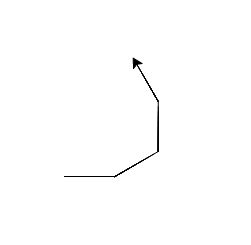
\includegraphics[width=0.4\linewidth]{turtleExample.png}
            \caption{Interpretacja dla słowa $\alpha\beta\alpha\beta\beta\alpha\beta\alpha$, gdzie $\alpha$ to idź naprzód, a $\beta$ skręć w lewo o 30\degree.}
            \label{fig:turtleExample}
        \end{figure}
        
        Aby żółw był w stanie rysować rośliny potrzebujemy symbol pozwalający się rozgałęziać. Można osiągnąć to poprzez dodanie stosu pamiętającego aktualny stan żółwia oraz symbole na nim operujące:
        \begin{description}[itemsep=2pt, parsep=2pt, topsep=2pt, partopsep=2pt]
            \item[{[}] -- odłóż aktualny stan na stos
            \item[{]}] -- ściągnij i zaaplikuj stan z góry stosu 
        \end{description}
        Stanem żółwia jest wszystko co zmienia się przy pomocy symboli np. pozycja, orientacja lub długość rysowanej linii. Rysunek \ref{fig:lsystemPlants} pokazuje przykładowe L--systemy z książki \textit{The Algorithmic Beauty of Plants}  \cite{plants}, które używają symboli tworzących rozgałęzienia. 
        \begin{figure}[H]
            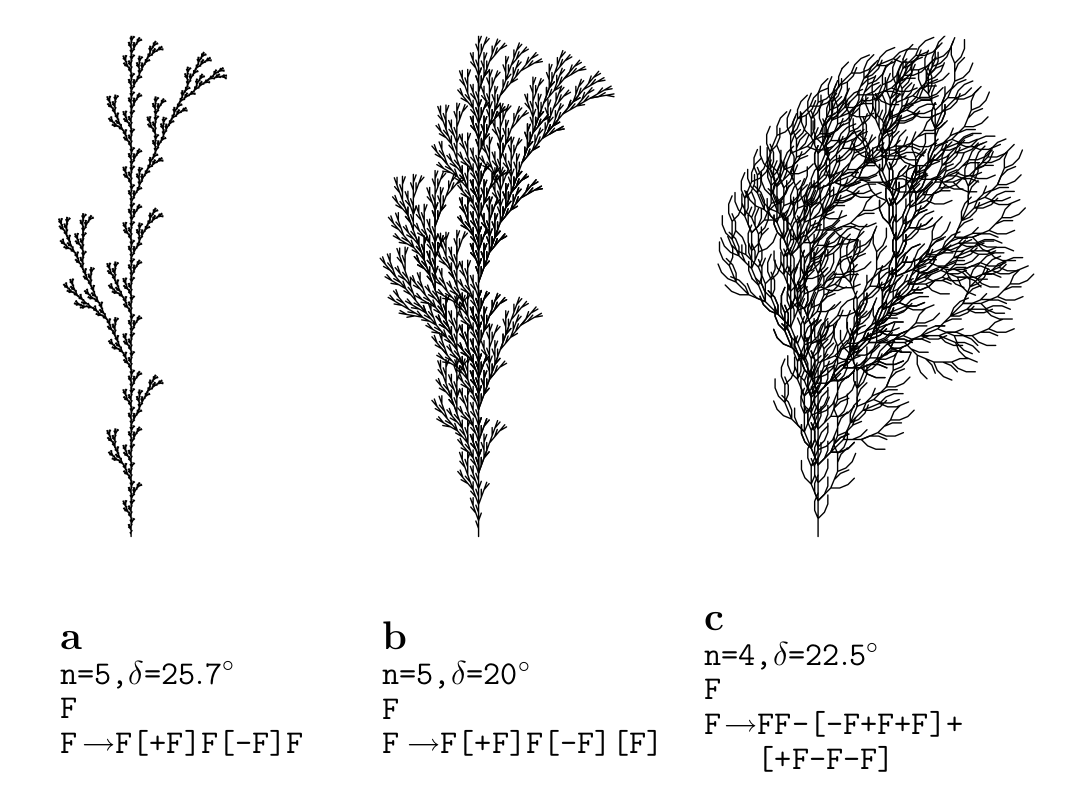
\includegraphics[width=\linewidth]{lsystemPlants.png}
            \caption{Przykład użycia symboli operujących na stosie \cite{plants}} 
            \label{fig:lsystemPlants}
        \end{figure}
        
        Wspomniana wcześniej książka Prusinkiewicza i Lindenmayer'a \cite{plants} dokładnie opisuje L--systemy jako zagadnienie naukowe oraz podaje wiele przykładów produkcji tworzących realistycznie wyglądające rośliny. Część z nich wymaga bardziej zaawansowanych technik produkcji symbolów np. L--systemy parametryczne. Do tej pory zakładaliśmy, że wszystkie parametry (np. kąt skrętu, długość kroku) były ustalone na początku i nie zmieniały się. Parametryzując symbole i produkcje możemy wpływać lepiej na finalny kształt. Ma to zastosowanie między innymi w generowaniu drzew. Rysunek \ref{fig:hondaTrees} przedstawia produkcje drzew wymyślonych przez Hondę \cite{honda}, a pokazanych u Prusinkiewicza \cite{plants}.
        \begin{figure}[H]
            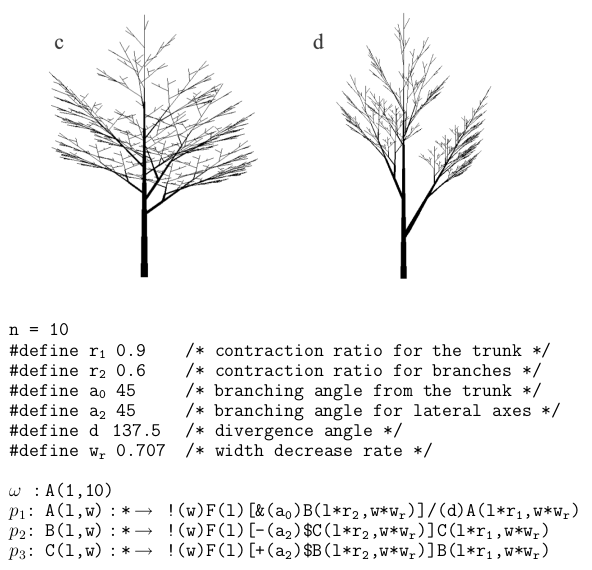
\includegraphics[width=\linewidth]{hondaTrees.png}
            \caption{L--system parametryczny generujący drzewa \cite{plants}\cite{honda}} 
            \label{fig:hondaTrees}
        \end{figure}
        
        L--systemy mogą również generować wielokąty. Jest to szczególnie przydatne w tworzeniu liści. Rysunek \ref{fig:lsystemLeafs} prezentuje kilka rodzajów liści wygenerowanych z jednego L--systemu. Możliwe jest to dzięki wprowadzeniu nowych symboli:
        \begin{description}[itemsep=2pt, parsep=2pt, topsep=2pt, partopsep=2pt]
            \item[\text{\{}] -- zacznij tworzyć nowy wielokąt 
            \item[.] -- zapisz aktualną pozycję jako wierzchołek
            \item[\text{\}}] -- zakończ aktualny wielokąt
        \end{description}
        \begin{figure}[H]
            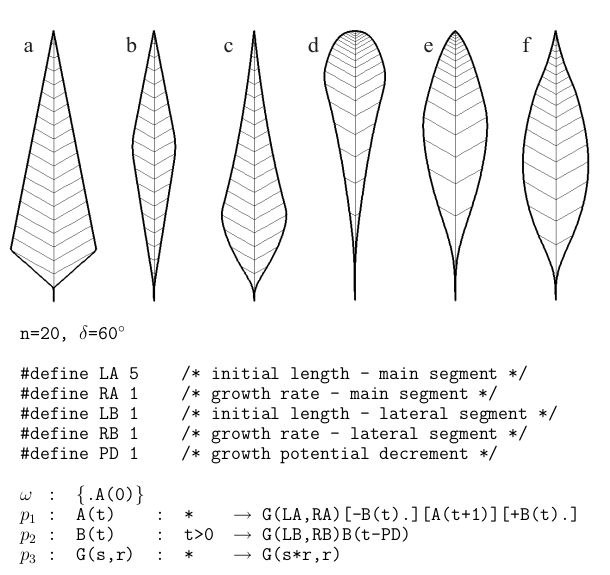
\includegraphics[width=\linewidth]{lsystemLeafs.png}
            \caption{L--system parametryczny generujący liście \cite{plants}.} 
            \label{fig:lsystemLeafs}
        \end{figure}
        
        Wcześniej opisane zastosowania L--systemów pokazują dlaczego jest to idealny kandydat do tworzenia realistycznych modeli roślin. Różnorodność definiowanych kształtów, rozbudowywanie funkcjonalności poprzez dodawanie nowych symboli oraz łatwe parametryzowanie to jedne z wielu zalet tej techniki. Wszystko to sprawia, że L--systemy są często wykorzystywane w wielu różnych projektach -- również w tym. 
        
    \section{Teren}
        Problem generowania terenu można sprowadzić do problemu generowania mapy wysokości. Jest to macierz wypełniona liczbami reprezentującymi wysokość wybranych punktów. Owe punkty pomiaru rozłożone są równomiernie na osi $X$ i $Z$. Mając taką macierz w łatwy sposób jesteśmy w stanie wygenerować teren -- tworzymy kwadraty dla każdej czwórki sąsiadujących punktów (rysunek \ref{fig:heightmap}). 
        \begin{figure}[H]
            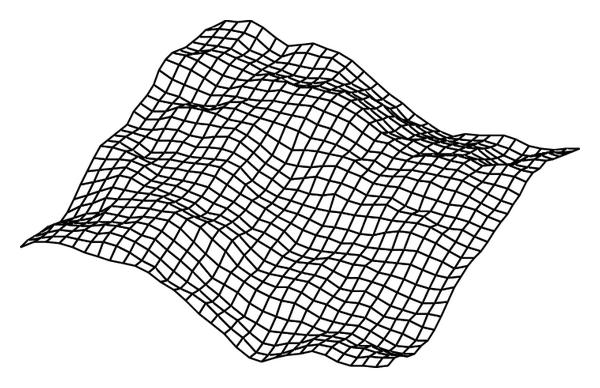
\includegraphics[width=\linewidth]{heightmap.png}
            \caption{Przykładowy teren wygenerowany przy użyciu mapy wysokości \cite{heightmap}} 
            \label{fig:heightmap}
        \end{figure}
        
        Istnieje wiele algorytmów generujących mapy wysokości. W programie użyto tak zwanego \textit{Diamond--square algorithm}. Dla ustalonego N generuje on mapę wysokości o rozmiarze $2^N$+1 x $2^N$+1. Na początku ustala się wartości w rogach macierzy. Następnie wykonuje się na przemiennie fazę diamond i square, aż do ustalenia wszystkich wysokości. 
        
        Faza diamond polega na wygenerowaniu wysokości w środku każdego kwadratu, który nie ma ustalonej wartości. Faza square robi to samo tylko, że dla punktów tworzących kształt rombu. Rysunek \ref{fig:diamondSquare} obrazuje przebieg algorytmu. 
        \begin{figure}[H]
            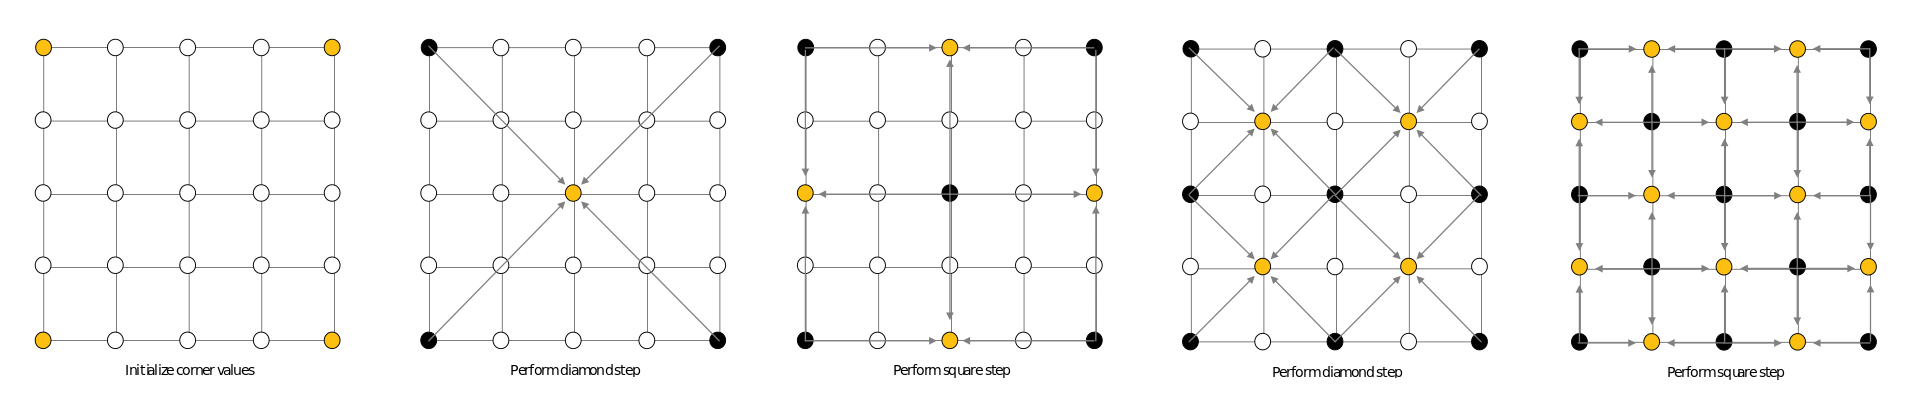
\includegraphics[width=\linewidth]{diamondSquare.png}
            \caption{Przebieg algorytmu diamond--square dla N = 2.} 
            \label{fig:diamondSquare}
        \end{figure}
        
        Obliczanie nowej wartości w środku polega na wzięciu średniej z wysokości wierzchołków tworzących kształt (kwadrat, romb). Dodatkowo dodajemy do obliczanej wartości pewien czynnik losowy z przedziału $(-X, X)$ dla ustalonego $X$. Dla każdej kolejnej pary faz ów czynnik jest zmniejszany poprzez przemnożenie go przez ustalone $R < 1$.
        
        \textit{Diamond--square algorithm} jest zarówno prosty jak i efektywny. Ustalając kilka parametrów jesteśmy w stanie tworzyć bardzo różnorodny teren. W łatwy sposób możemy wpływać na dokładność modelu oraz kształt. Wszystko to sprawia, że ten algorytm jest dobrym kandydatem do generowania terenu.
        
    \section{Tekstury}
        Aby wygenerowany model był kompletny poza kształtem musimy również nadać mu kolor. Jednym z założeń programu było w pełni proceduralne podejście. Dotyczy to również tekstur. Każda tekstura w programie opisywana jest przez materiał. Materiał oblicza kolor na podstawie funkcji \textit{calcDiffuse(pos3D) \textrightarrow color}, gdzie $pos3D$ to pozycja w świecie. W celu uproszczenia i ujednolicenia systemu zaimplementowano jeden wzór, który został zastosowany do każdego materiału. Wygląda on następująco:
        \begin{gather*} \label{eqn:material}
            calcDiffuse(pos3D) = mix(color1, color2, factor) \\
            gdzie \\
            factor = clamp(noise(pos3D * posF) * valF, 0, 1)
        \end{gather*}
        

        Finalny kolor to mieszanka $color1$ i $color2$ w stosunku $1 - factor$ i $factor$. Sam $factor$ to odpowiednio obliczona wartość szumu Perlina \cite{perlinNoise}. Dzięki $posF$ możemy skalować szum, a dzięki $valF$ możemy wymuszać faworyzowanie wartości bliższych 0 albo 1.
        
        Jedynym materiałem w programie odbiegającym od tej metody jest materiał terenu. Łączy on ze sobą dwa inne materiały -- grunt i skały. Do pewnej ustalonej wysokości kolor obliczany jest tylko dla gruntu. Analogicznie powyżej pewnego poziomu aplikowany jest tylko kolor skał. Po środku dochodzi do mieszania kolorów w stosunku zależnym od odległości do ustalonych granic:
        \begin{gather*}
        mix(calcRockColor(pos), calcGroundColor(pos), groundFactor) \\
        gdzie \\
        groundFactor = (groundEndY - posY) / (groundEndY - rockStartY) \\
        \end{gather*}
        
        Zaprezentowane rozwiązanie okazało się wystarczające, aby osiągnąć zadowalające rezultaty. Jest łatwe do implementacji, ujednolicone dla użytkownika oraz na tyle rozbudowane, aby wyrażać niebanalną kolorystkę.
        
    \section{Rozmieszczanie roślin}
        Po wygenerowaniu wystarczającej liczby modeli roślin trzeba je umieścić w świecie. Można to robić w mniej lub bardziej wyszukany sposób. W tym przypadku zastosowano jedno z najprostszych rozwiązań -- losowe rozmieszczanie wewnątrz komórek kraty. Krata o wymiarach $N$ x $M$ posiada $N * M$ kwadratowych komórek o ustalonym rozmiarze. Wewnątrz takiej komórki z pewnym prawdopodobieństwem możemy umieścić losowy model. Pozycja modelu wewnątrz kraty również jest losowa i może zostać ograniczona przez parametr mówiący jak bardzo od środka może zostać wylosowana. Przykładowo dla wartości 0 obiekt zawsze będzie umieszczany w środku kraty, a dla 1 może pojawić się w całej kracie. 
        
    \section{Ograniczenie liczby modeli}
        Przy generowaniu tak dużego świata musimy liczyć się z ograniczeniami sprzętowymi. Niezoptymalizowane modele otrzymywane z L--systemów mają nawet po kilkanaście tysięcy trójkątów! W takim przypadku dobrym sposobem tworzenia sceny jest umieszczenia wszystkich generowanych modeli względnie blisko kamery, która renderuje obraz. Duże modele będą zasłaniać znaczną część pola widzenia ukrywając niewypełnioną przestrzeń. Rozwiązanie nie jest idealne ale ma szanse wygenerować scenę o zadowalającym rezultacie. To podejście ma swoje odwzorowanie w implementacji rozmieszczania roślin, które jest robione zależnie od położenia kamery.
        
\chapter{Realistyczny rendering}
    Do tej pory przyjrzeliśmy się technikom pozwalającym generować różne modele składające się w jeden wielki świat. W tej sekcji skupimy się jak uchwycić część tego co udało się stworzyć. Sam proces zwany renderingiem w tym przypadku przypominać będzie nic innego jak zrobienie zdjęcia. Wcześniej pojawiło się pojęcie kamery. Jest to niewidoczny obiekt umieszczony w świecie, zwrócony w określonym kierunku. To co należy zrobić to uchwycić obraz z jego perspektywy. 
    
    \section{Path tracer}
        Głównym zadaniem path tracer'a jest obliczanie koloru docierającego do kamery z ustalonego kierunku. Kolor w tym przypadku to nic innego jak promień światła, który po wielu odbiciach dotarł do kamery. Postaramy odtworzyć się to zjawisko, z tym wyjątkiem, że promień zostanie wypuszczony od kamery i będzie podążać do światła. Cały proces jest wysoce losowy, jako że promień mógł dotrzeć do nas wieloma różnymi ścieżkami. W celu otrzymania jak najlepszych wyników w jednym kierunku będziemy puszczać wiele promieni, a na końcu je uśrednimy.
        
        Aby otrzymać realistyczny obraz, path tracer przy obliczaniu koloru będzie korzystać z tak zwanego \textit{równania renderingu} \cite{pbrt}. Samo równanie korzystając z zasady zachowania energii wylicza radiancję światła wychodzącą z ustalonego punktu na płaszczyźnie dla zadanego kierunku. Wygląda ono następująco:
        
        \begin{equation*}
            L_o(p, \omega_o) = L_e(p, \omega_o) + \int_{\Omega} f_r(p, \omega_o, \omega_i) * L_i(p, \omega_i)*cos\theta_i*d\omega_i
        \end{equation*}
        
        gdzie:
        
        \begin{description}
            \item[$p$] -- punkt przecięcia promienia z płaszczyzną
            \item[$\omega_o$] -- kierunek wychodzącego światła
            \item[$\omega_i$] -- ujemny kierunek przychodzącego światła
            \item[$\Omega$] -- półsfera położona na płaszczyźnie zawierające wszystkie wartości $\omega_i$ 
            \item[$L_o(p, \omega_o)$] -- radiancja spektralna wychodząca z punktu $p$ w kierunku $\omega_o$
            \item[$L_e(p, \omega_o)$] -- radiancja spektralna emitowana przez płaszczyznę w kierunku $\omega_o$ z punktu $p$  
            \item[$f_r(p, \omega_o, \omega_i)$] -- dwukierunkowa funkcja rozkładu odbicia (BRDF)
            \item[$L_i(p, \omega_i)$] -- radiancja spektralna przychodząca z kierunku $\omega_i$ do punktu $p$
            \item[$cos\theta_i$] -- współczynnik osłabiający zależny od kierunku przychodzącego promienia $\omega_i$ i wektora normalnego płaszczyzny
        \end{description}

        Rysunek \ref{fig:renderingEquation} przedstawia sytuację obliczania radiancji dla ustalonego promienia przychodzącego.
        
        \begin{figure}[H]
            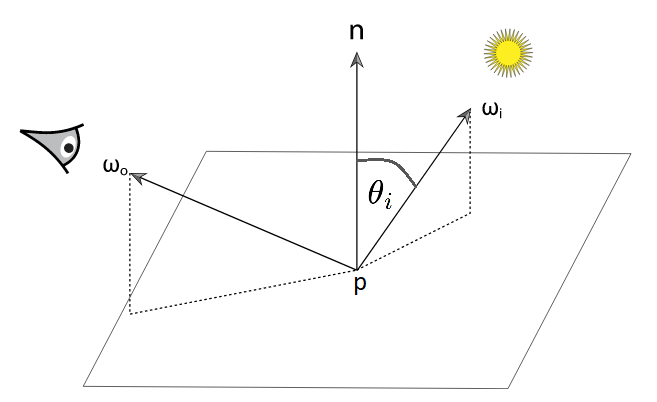
\includegraphics[width=\linewidth]{renderingEquation.png}
            \caption{Sytuacja obliczania radiancji dla ustalonego promienia przychodzącego \cite{pbrt}.} 
            \label{fig:renderingEquation}
        \end{figure}
        
    \section{Niebo}
        Path tracing często stosuje się dla zamkniętych scen z kilkoma źródłami światła. W przypadku renderowania krajobrazów mamy do czynienia z czymś zupełnie innym -- jedno źródło światła (słońce) oraz pół otwarta scena z wielkim niebem pochłaniającym większość promieni. Fizycznie poprawny model nieba został opisany w pracy  A. J. Preetham'a, 
        Peter Shirley'a i Brian Smits'a pod tytułem \textit{A Practical Analytic Model for Daylight} \cite{sky}, która powstała na Uniwersytecie w Utah. Model opisuje niebo w danym miejscu na ziemi o ustalonej porze. 
        
        Został również udostępniony gotowy kod implementujący zaprezentowane rozwiązanie. Dołączony do programu, wykorzystywany jest jak zewnętrzna biblioteka bez wnikania w szczegóły implementacyjne. Niebo w programie to półsfera rozciągająca się nad całym wygenerowanym terenem. Implikuje to, że im większy jest teren, tym większe jest niebo.
    
    \section{Słońce}
        O ile model nieba z poprzedniej sekcji dobrze oddaje kolorystykę nieba, to jest ona dosyć jednolita. Dodatkowo jako, że niebo otacza scenę praktycznie z każdej strony, to nie może być traktowane jako główne źródło światła. Żeby otrzymać realistyczne cienie obiektów dołożono dodatkowo słońce jako źródło światła o dużej mocy. Umieszczane jest zgodnie z wyliczeniami z modelu nieba. Znajduje się na półsferze nieba stąd odległość słońca od ziemi jest zależna od wielkości terenu (patrz poprzednia sekcja).
        
    \section{Wybór miejsca renderingu}
        Aby teren wydawał się realistyczny musi zajmować dużą część świata. Dobrze byłoby wpływać na to czy chcemy renderować naszą scenę ze szczytu góry czy z terenu nizinnego. W jakim kierunku powinna być skierowana kamera oraz co ważniejsze uwzględniać ukształtowanie otaczającego ją terenu. W przypadku gdy kamera zostanie umieszczona przed górą chcielibyśmy, aby patrzyła do góry, a kiedy jest na szczycie w dół. 
        
        Odpowiednie umieszczenie możemy wybrać poprzez parametr sugerujący na jakiej wysokości chcemy się znajdować. Dobrze zdefiniować również minimalną odległość od krawędzi końca świata, aby uniknąć sytuacji patrzenia w pustą przestrzeń. Żeby uwzględnić ukształtowanie terenu przy kierunku patrzenia możemy dodać parametr, mówiący jak daleko od nas znajduję się miejsce, które nas interesuje. Następnie obliczamy wysokość tego miejsca i korygujemy nasz kierunek patrzenia względem otrzymanej wartości.
        
\chapter{Poradnik użytkowania}
    W poprzednich dwóch rozdziałach opisano rozwiązania zastosowane w programie. Ten skupi się jak go uruchomić oraz przedstawi w jaki sposób wpływać na rendering i generowane elementy.
    
    \section{Uruchomienie programu}
        Program był pisany i testowany na systemie operacyjnym \textit{Ubuntu 18.04}. Użyty język programowania to \textit{C++14}.
        Repozytorium można sklonować z adresu: \url{https://github.com/bratek20/RPForest}.
        
        Program korzysta z następujących narzędzi i bibliotek:
        \begin{itemize}
            \item \textit{cmake}
            \item \textit{GLM}
            \item \textit{GLEW}
            \item \textit{GLFW3}
            \item \textit{Embree3}
            \item \textit{OpenEXR}
        \end{itemize}

        
        W celu instalacji programu należy uruchomić skrypt \textit{install.sh} w głównym katalogu. Skrypt instaluje wszystkie wymagane biblioteki oraz przydatne narzędzia. Na końcu uruchamia skrypt budujący program -- \textit{build.sh}. Tworzy on folder \textit{build}, który posłuży jako miejsce dla plików programu \textit{cmake} i go uruchamia. Na końcu w folderze \textit{bin} pojawi się plik binarny programu -- \textit{rpforest.exe}. Należy uruchomić go z linii poleceń. Program posiada dwa opcjonalne argumenty wywołania. 
        
        Pierwszy to nazwa folderu z plikami konfiguracyjnymi. Katalog musi znajdować się w folderze \textit{configs}. Znajduje się tam domyślna konfiguracja \textit{default}, która jest wczytywana jeśli użytkownik nie poda żadnego argumentu. 
        
        Drugi argument to ziarno losowości. W przypadku nie ustawienia żadnego, zostanie wybrane losowe -- zależne od czasu. W logach programu można znaleźć ziarno dla danego uruchomienia. Możemy wybrać je podobnie jeśli chcemy wygenerować ten sam świat. 
    
    \section{Tryb zwykły i debugowania}
        Program ma dwa tryby: zwykły i debugowania. 
        
        Tryb zwykły po uruchomieniu od razu generuje finalny obraz i kończy działanie. 
        
        Tryb debugowania otwiera okno wyświetlające wygenerowany świat. Widzimy go z pozycji kamery. Możemy poruszać się w świecie w celu wyboru lepszego miejsca renderingu i wygenerować finalny obraz klikając odpowiedni przycisk na klawiaturze. Wyświetlany obraz w trybie debugowania różni się od generowane finalnego obrazu. Wynika to z faktu zastosowania zupełnie innej technologi, w celu płynnego wyświetlania świata w czasie rzeczywistym.
        
        Pełny opis możliwych akcji:
        \begin{itemize}
            \item zmiana kierunku patrzenia kamery -- ruch myszką
            \item poruszanie kamerą -- W (przód), S (tył), A (lewo), D (prawo) lub odpowiednie strzałki
            \item rendering aktualnego widoku -- przycisk P
            \item wypuszczenie testowych promieni -- przycisk L. Po naciśnięciu przycisku w kierunku patrzenia kamery, zostanie wystrzelone kilka promieni. Liczba promieni oraz liczba odbić każdego z nich jest zależna od ustawień path tracingu.
        \end{itemize}
        
    \section{Pliki konfiguracyjne}
        Każdy plik konfiguracyjny jest parsowany w ten sam sposób. Pojedynczy wpis składa się z nazwy parametru i argumentów zależnych od typu parametru. Kolejność nie ma znaczenia. Każdy parametr musi być zdefiniowany w osobnej linii. Część parametrów ma domyślne wartości. 
        
        Wszystkie pliki powinny znajdować się w katalogu umieszczonym w folderze \textit{configs}, którego nazwa została podana jako pierwszy argument programu. Ich rozszerzenia oraz umieszczenie w podfolderach ma znaczenie.
        
        Poniżej zostaną opisane parametry poszczególnych plików konfiguracyjnych, ich lokalizacja oraz zastosowanie. Przyjęta konwencja to:
        \begin{itemize}
            \item \textit{NazwaParametru : typ = wartość domyślna jeśli istnieje} -- opis
        \end{itemize}
        
        Jeśli nie jest sprecyzowana nazwa pliku, a jedynie rozszerzenie to znaczy, że może być wiele plików konfigurującą daną funkcjonalność. W takim przypadku użytkownik może tworzyć nowe pliki lub usuwać istniejące.
        
        \subsection{Ustawienia path tracingu}
        Plik opisujący path tracing umieszczony jest w głównym folderze konfiguracyjnym i ma nazwę \textit{pathTracer.conf}.
        
        Można zdefiniować następujące parametry:
        \begin{itemize}
            \item \textit{PhotoName : string} -- nazwa pliku do którego zostanie zapisany finalny render. Będzie on w formacie exr i umieszczony zostanie w folderze \textit{photos}.
            \item \textit{Resolution : vec2} -- rozmiar renderowanej fotografii
            \item \textit{Samples : int = 1} -- liczba promieni wystrzelona per jeden pixel
            \item \textit{MaxRayBounces : int = 5} -- maksymalna dopuszczalna liczba odbić jednego promienia  
        \end{itemize}

        \subsection{Ustawienia kamery}
        Plik opisujący ustawienia kamery z głównego folderu: \textit{camera.conf}.
        
        Parametry:
        \begin{itemize}
            \item \textit{LookHeight : float = 1} -- wysokość liczona od  powierzchni ziemi 
            \item \textit{LookDirection : vec3 = 0 0 1} -- kierunek patrzenia 
            \item \textit{LookDistance : float = 2} -- odległości od kamery, względem której zostanie dostosowane pochylenie kamery (patrzenie pod góre/w dół)
            \item \textit{EdgeMinOffset : float = 10} -- minimalna odległość od krawędzi świata  
            \item \textit{ExpectedPositionY : float = 0} -- oczekiwana pozycja Y, na której powinna zostać umieszczona kamera. Dzięki temu można wymuszać np. robienie zdjęć ze szczytów gór poprzez ustawienie bardzo dużej wartości (kamera zawsze będzie \textit{LookHeight} nad ziemią). 
        \end{itemize}
        
        \subsection{Ustawienia debugowania}
        Plik do zmiany ustawień debugowania znajdujący się w głównym folderze: \textit{debug.conf}.
        
        Parametry:
        \begin{itemize}
            \item \textit{Enabled : bool = false} -- czy jest włączony tryb debugowania
            \item \textit{Resolution : vec2 = 800 600} -- rozmiar okna debugowania
            \item \textit{CameraVelocity : float = 10} -- prędkość poruszania się kamery 
        \end{itemize}
        
        \subsection{Ustawienia nieba}
        Plik do konfiguracji nieba z głównego folderu: \textit{sky.conf}. Większość parametrów służy do ustawień modelu nieba opracowanego w pracy z Uniwersytetu w Utah \cite{sky}.
        
        Parametry słońca:
        \begin{itemize}
            \item \textit{SunColor : vec3} -- kolor słońca 
            \item \textit{SunPower : float} -- moc słońca
        \end{itemize}
        
        Parametry modelu nieba:
        \begin{itemize}
            \item \textit{SkyLuminanceFactor : float} -- mnożnik do zmniejszania jasności pochodzącej od nieba
            \item \textit{Latitude : float} -- szerokość geograficzna
            \item \textit{Longitude : float} -- długość geograficzna
            \item \textit{StandardMeridian : int} -- numer strefy czasowej
            \item \textit{JulianDay : int} -- dzień
            \item \textit{TimeOfDay : float} -- czas
            \item \textit{Turbidity : float} -- zagęszczenie mgły 
        \end{itemize}
        
        \subsection{Ustawienia terenu}
        Ustawienia terenu wpływające na algorytm \textit{diamond--square} oraz teksturowanie są opisane w pliku: \textit{terrain.conf} umieszczonym w głównym folderze.
        
        \begin{itemize}
            \item \textit{N : int} -- wpływa na liczbę elementów mapy wysokości. Finalny rozmiar to $2^N+1$ x $2^N+1$.
            \item \textit{Size : float} -- wielkość generowane terenu 
            \item \textit{InitHeight : float} -- wartość do wyliczania początkowych wartości na rogach mapy. Zostaną wylosowane z przedziału $(-\textit{InitHeight}:\textit{InitHeight})$.
            \item \textit{Spread : float} -- początkowa rozpiętość losowej wysokości dodawanej do uśrednianych wartości. Losowa wysokość losowana jest z przedziału $(-\textit{Spread}:\textit{Spread})$, gdzie \textit{Spread} będzie maleć z każdą iteracją algorytmu.
            \item \textit{SpreadReductionRate : float} -- jak zmienia się rozpiętość wzgledem kolejnych iteracji algorytmu. Parametr powinien mieć wartość mniejszą niż 1. 
            \item \textit{RockStartY : float = 10} -- od jakiej wysokości powinien być aplikowany materiał skał
            \item \textit{GroundEndY : float = 20} -- do jakiej wysokości powinien być aplikowany materiał gruntu. Parametr powinien mieć wartość większą niż \textit{RockStartY}. 
        \end{itemize}
        
        \subsection{Ustawienia tekstur}
        Wszystkie pliki konfiguracyjne materiałów znajdują się w folderze \textit{materials} i mają rozszerzenie \textit{.mat}. W plikach ustala się wartości parametrów ze wzoru \ref{eqn:material}. 
        \begin{itemize}
            \item \textit{Color1 : vec3} -- pierwszy kolor do mieszania
            \item \textit{Color2 : vec3} -- drugi kolor do mieszania
            \item \textit{NoisePositionFactor : float = 1} -- czynnik zmieniający pozycję obliczania szumu 
            \item \textit{NoiseValueFactor : float = 1} -- czynnik zmieniający wartość szumu
        \end{itemize}
        
        \subsection{Bazowe ustawienia generatorów}
        Program pozwala definiować własne L--systemy oraz udostępnia kilka predefiniowanych. Oba podejścia konfigurowane są przez odpowiednie pliki, które współdzielą część parametrów:
        
        \begin{itemize}
            \item \textit{N : int} -- liczba iteracji aplikowania produkcji L--systemu 
            \item \textit{Height : float} -- finalna wysokość wygenerowanego modelu
            \item \textit{ConeBasePoints : int = 3} -- ile punktów w podstawie mają cylindry tworzące model
            \item \textit{Material : string} -- nazwa materiału (Leaf, Bark, Plant)
            \item \textit{InitRadius : float} -- początkowy promień cylindrów tworzących model. Finalnie model jest przeskalowany tak by miał wysokość \textit{Height}, więc ten parametr służy do zmieniania stosunku grubości do wysokości. 
        \end{itemize}
        
        \subsection{Definiowanie własnych L--systemów}
        Wszystkie pliki definiujące własne L--systemy mają rozszerzenie \textit{.lsys}. Można umieścić je w jednym z trzech folderów: \textit{trees}, \textit{plants} albo \textit{leafs}. Umieszczenie wpływa na to jak program będzie traktować dany L--system.
        
        \begin{itemize}
            \item \textit{TurnAngle : float = 0} -- kąt skrętu żółwia w lewo/prawo
            \item \textit{PitchAngle : float = 0} -- kąt skrętu żółwia w dół/górę 
            \item \textit{RollAngle : float = 0} -- kąt skrętu wokół własnej osi
            \item \textit{Axiom : char} -- początkowy symbol
            \item \textit{Prod : char $>$ string } -- pojedyncza definicja produkcji. Plik może zawierać kilka takich wpisów (każdy w osobnej linii) i wszystkie zostaną uwzględnione. Poprawny zapis to symbol, znak $>$ (dla lepszej czytelności) i produkowane słowo np. \textit{Prod A $>$ ABC}. 
        \end{itemize}
        
        Dostępne symbole sterujące żółwiem to:
        \begin{itemize}
            \item \textit{F} -- idź w przód tworząc cylinder
            \item \textit{f} -- idź w przód
            \item {[} -- rozpocznij tworzenie gałęzi
            \item {]} -- zakończ tworzenie gałęzi
            \item + -- obróć się w prawo o \textit{TurnAngle}
            \item --- -- obróć się w lewo o \textit{TurnAngle}
            \item \^{} -- obróć się w górę o \textit{PitchAngle}
            \item \& -- obróć się w dół o \textit{PitchAngle}
            \item \textbackslash -- obróć się wokół osi zgodnie z ruchem wskazówek zegara o \textit{RollAngle}
            \item \text{/} -- obróć się wokół osi przeciwnie do ruchu wskazówek zegara o \textit{RollAngle}
            \item $|$ -- obróć się w lewo o 180\degree
            \item \textbraceleft -- zacznij tworzyć wielokąt
            \item . -- zapisz aktualną pozycję jako wierzchołek wielokąta
            \item \textbraceright -- skończ tworzyć wielokąt
        \end{itemize}
        
        \subsection{Ustawienia predefiniowanych L--systemów}
        W programie zostały zaimplementowane dwa L--systemy: jeden do generowania drzew, drugi do liści.
        
        Pliki konfiguracyjne do generowania drzew mają rozszerzenie \textit{.honda} i muszą znajdować się w folderze \textit{trees}. Opisują one wartość L--systemu wymyślonego przez Hondę \cite{honda} i zaprezentowanego przez Prusinkiewicza \cite{plants} -- patrz Rysunek \ref{fig:hondaTrees}.
        
        Parametry z rysunku z dokładnością do wielkości liter:
        \begin{itemize}
            \item \textit{R1 : float} -- współczynnik zmniejszania długości pnia
            \item \textit{R2 : float} -- współczynnik zmniejszania długości gałęzi
            \item \textit{A0 : float} -- kąt pod którym rosną gałęzie
            \item \textit{A2 : float} -- kąt pod którym wyrastają pomniejsze gałęzie
            \item \textit{D : float} -- kąt o ile rotuje wokół własnej osi żółw po stworzeniu gałęzi
            \item \textit{Wr : float} -- współczynnik zmniejszania promienia pnia i gałęzi
        \end{itemize}    
        
        Przykładowy L--system tworzący liście został przedstawiony na rysunku \ref{fig:lsystemLeafs}. Pliki go opisujące mają rozszerzenie \textit{.family} i umieszczone są w folderze \textit{leafs}. Zawierają:
        \begin{itemize}
            \item \textit{Delta : float} -- kąt skrętu żółwia w lewo/prawo
            \item \textit{LA : float} -- początkowa długość głównego segmentu
            \item \textit{RA : float} -- współczynnik wzrostu głównego segmentu
            \item \textit{LB : float} -- początkowa długość bocznych segmentów
            \item \textit{RB : float} -- współczynnik wzrostu bocznych segmentów
            \item \textit{PD : float} -- ubytek rośnięcia bocznych fragmentów
        \end{itemize}    
        
        \subsection{Ustawienia rozmieszczania roślin}
        Grupy elementów można umieszczać w świecie przy pomocy plików o rozszerzeniu
        \textit{.spawner} umieszczonych w folderze \textit{sprawners}.
        \begin{itemize}
            \item \textit{CameraOffset : vec2} -- przesunięcie środka kraty względem pozycji kamery
            \item \textit{XGridN : int = 1} -- liczba komórek kraty wzdłuż osi X
            \item \textit{ZGridN : int = 1} -- liczba komórek kraty wzdłuż osi Z
            \item \textit{CellSize : float = 0} -- rozmiar pojedynczej komórki
            \item \textit{GeneratorType : string} -- typ użytego generatorów (Tree, Plant)
            \item \textit{SpawnProbability : float = 1} -- szansa na stworzenie pojedynczego elementu 
            \item \textit{RandomPositionPercentage : float = 0.5} -- na jak dużym obszarze wokół środka komórki mogą być tworzone elementy
            \item \textit{MinElementScale : float = 0.5} -- minimalna wartość, która może zostać wybrana do skalowania pojedynczego elementu
            \item \textit{MaxElementScale : float = 2} -- maksymalna wartość, która może zostać wybrana do skalowania pojedynczego elementu
        \end{itemize}
    
        
\chapter{Szczegóły programistyczne}
    \section{Wykaz użytych narzędzi}
        Program napisany jest w języku \textbf{C++}. Można w nim pisać obiektowo, a zarazem dbać o efektywność programu. Dostępne jest wiele bibliotek graficznych, które są dobrze udokumentowane. Z uwagi na popularność języka w przypadku jakichkolwiek trudność, łatwo można znaleźć materiały z propozycją rozwiązania problemu.        
        
        Większość obliczeń matematycznych korzysta z typów i operacji zawartych w bibliotece \textbf{GLM}. Jest to mała i prosta w użyciu biblioteka zawierająca wszystkie przydatne funkcje matematyczne. Udostępnia również typy takie jak \textit{vec3} lub \textit{mat4}, które są często używane w grafice komputerowej. 
        
        Tryb debugowania korzysta z OpenGL w celu wyświetlania świata. Użyte biblioteki to \textbf{GLEW} oraz \textbf{GLFW3}. Są one ogólnie dostępne, dobrze udokumentowane i łatwe w użyciu. 
        
        Path tracer korzysta z biblioteki \textbf{Embree3}. Pozwala ona w bardzo szybki sposób obliczać przecięcia promieni z trójkątami, co jest kluczowym elementem path tracingu. 
        
        Do tworzenia obrazów w formacie \textit{.exr} wykorzystana została biblioteka \textbf{OpenEXR}. Format zapisu pozwala na manipulowanie wieloma parametrami wygenerowanego obrazu w celu poprawienia wyglądu. 
        Pliki w tym formacie można wyświetlić np. przy pomocy programu \textit{exrdisplay}.
        
    \section{Struktura projektu}
        Program składa się z czterech modułów:
        \begin{itemize}
            \item \textit{engine} -- baza całego programu, przypominająca silnik 3D. Implementuje podstawowe funkcjonalności wykorzystywane i rozszerzane przez inne moduły. 
            \item \textit{rendering} -- moduł implementujący wszystkie zagadnienia związane z path tracingiem
            \item \textit{generating} -- moduł implementujący wszystkie zagadnienia związane z generowaniem proceduralnym
            \item \textit{utils} -- moduł implementujący niezależne lub pomocnicze funkcjonalności
        \end{itemize}
        
        \subsection{Moduł \textit{engine}}
            Zarówno rendering przy pomocy OpenGL jak i techniką path tracingu wymaga reprezentacji obiektu, który ma renderować. Podstawowym sposobem opisów złożonych kształtów jest przedstawienie ich przy pomocy zbioru trójkątów. Każdy trójkąt (klasa \textbf{Triangle}) składa się z trzech wierzchołków (klasa \textbf{Vertex}), które poza pozycją w świecie zawierają takie informacje jak wektory normalne (reprezentujące orientację w przestrzeni). Pojedynczy zbiór trójkątów trzymany jest w obrębie obiektu klasy \textbf{Mesh}, która dodatkowo definiuje kolorystykę reprezentowanego kształtu przy pomocy materiału (klasa \textbf{Material}). Finalny model (klasa \textbf{Model}) to zbiór mesh'y. Pozwala to wyrazić dowolnie skomplikowany (pod względem kształtu i kolorystki) obiekt. 
            
            Jedną z najważniejszych klas modułu jest \textbf{Actor}. Reprezentuje on dowolny obiektu w świecie. Aktor może mieć kształt opisany przy pomocy klasy \textbf{Model}. Posiada on dodatkowo zbiór parametrów pozwalający wpływać na finalną reprezentację np. pozycja, skala, rotacja. Dzięki temu możemy umieścić ten sam model w różnych miejscach w świecie i zmienić jego rozmiar.
            
            Cały świat reprezentowany przy pomocy klasy \textbf{Scene}. Scena to rodzaj aktora, który zbiera wszystkich innych aktorów, odpowiednio ich inicjalizuje i rozmieszcza. Jednym z aktorów umieszczonych na scenie jest między innymi kamera (klasa \textbf{Camera}). Scena wykorzystuje funkcjonalność aktora: relacja rodzic--dziecko. Każdy aktor może mieć niezerową liczbę dzieci. Wszystkie parametry rodzica wpływają na dziecko np. zmieniając pozycję rodzica, przemieścimy wszystkie jego dzieci oraz dzieci tych dzieci (wnuki) itd. Dodatkowo akcje jak aktualizowanie (funkcja \textbf{update}) albo renderowanie w trybie debugowania (funkcja \textbf{render}) działają pierw na rodzica, a następnie na jego wszystkie dzieci.
            
            Moduł implementuje dodatkowo wiele klas, bez których program nie mógłby funkcjonować:
            \begin{itemize}
                \item \textbf{Window} -- wyświetla okno trybu debugowania
                \item \textbf{Input} -- zbiera akcje użytkownika i pozwala na nie reagować
                \item \textbf{Assets} -- wczytuje zasoby potrzebne programowi (np. pliki konfiguracyjne) i udostępnia je innym częściom programu 
            \end{itemize}
            
        \subsection{Moduł \textit{rendering}}
            Najważniejsza klasa modułu to \textbf{PathTracer}. Implementuje ona obliczanie koloru pochodzącego z danego kierunku. Korzysta z dwóch pomocniczych klas:
            \begin{itemize}
                \item \textbf{AccStruct} -- interfejs struktury obliczającej przecięcie danego promienia z najbliższym trójkątem. Przykładowa implementacja to \textbf{EmbreeWrapper}, która wykorzystuje bibliotekę Embree do obliczania przecięć. 
                \item \textbf{SkyLightSampler} -- klasa obliczająca kolor nieba oraz próbkująca promienie pochodzące od słońca
            \end{itemize}
            
            Dodatkowo w głównym folderze modułu znajduje się podfolder \textit{ASky}, zawierający implementację modelu nieba udostępnioną przez pracowników z Uniwersytetu z Utah \cite{sky}.
            
        \subsection{Moduł \textit{generating}}
            Implementacje wszystkich zagadnień opisanych w pracy znajdują się w tym folderze. Duża część kodu zawiera implementację różnych symboli z L--systemów. Bazą jest klasa \textbf{Symbol}, która udostępnia dwie metody wirtualne: \textbf{vector \textless SymbolPtr \textgreater produce()} oraz \textbf{void process(ProcessContext\&)}. Pierwsza metoda służy do produkcji słowa dla aktualnego stanu symbolu. Pozwala to implementować zarówno parametryczne jak i losowe symbole. Druga metoda służy do wpływania na aktualny stan przetwarzania słowa z wygenerowanego L--systemu. Operuje ona na obiekcie struktury \textbf{ProcessContext}. Stuktura składuje między innymi: aktualny stan żółwia (klasa \textbf{Turtle}), stos odłożonych stanów żółwia (przy pomocy operatora rozgałęziania) oraz wygenerowany do tej pory model.
            
            Samo generowanie odbywa się w klasach pochodnych klasy \textbf{Generator}. Generator wymaga symbolu startowego oraz konfiguracji bazowej \textbf{GeneratorConfig}, aby wygenerować finalny model.
            
            Przykładowe klasy pochodne generatora to \textbf{LSysGenerator} albo \textbf{Honda}. Pierwszy implementuje obsługę plików konfiguracyjnych \textit{.lsys}, a drugi prezentuje implementację predefiniowanego L--systemu.
            
            Pozostałe klasy, na które warto zwrócić uwagę to:
            \begin{itemize}
                \item \textbf{DiamondSquareTerrain} -- klasa implementująca \textit{Diamond--square algorithm}. Udostępnia również metodę do obliczania wysokości terenu dla zdanego punktu oraz optymalnego umiejscowienia kamery.
                \item \textbf{SpawnerActor} -- specjalny rodzaj aktora, który rozmieszcza wygenerowane modele w zależności od konfiguracji z pliku \textit{.spawner} 
            \end{itemize}
            
        \subsection{Moduł \textit{utils}}
            Główna klasa modułu to \textbf{Utils}. Jest to klasa statyczna zawierająca wszystkie pomocnicze funkcje, wykorzystywane przez inne moduły. Dodatkowo posiada wiele stałych jak np. \textbf{PI} albo \textbf{INF}.
            
            Inne klasy modułu to:
            \begin{itemize}
                \item \textbf{Random} -- implementuje wiele losowych metod jak np. losowanie wektora na półsferze, obliczanie szumu perlina albo wybieranie elementu z tablicy
                \item \textbf{Timer} -- prosta klasa do mierzenia czasu  
            \end{itemize}
            
\chapter{Przykłady użycia}

\chapter{Porównanie z istniejącymi rozwiązaniami}

%%%%% BIBLIOGRAFIA

\bibliographystyle{unsrt}
\bibliography{bibliography}

%\begin{thebibliography}{1}
%\bibitem{example} \ldots
%\end{thebibliography}

\end{document}
